\chapter{Комплексні числа}


\section{Комплексні числа}

\begin{definition}
	\textbf{Комплексне число} --- це впорядкована пара дійсних чисел
	(компонент), для яких поняття рівності, суми, добутку вводяться наступним чином.
\end{definition}

\begin{enumerate}
	\item Нехай $z_1 = (x_1,y_1)$, $z_2 = (x_2,y_2)$. Тоді $z_1 = z_2 \Leftrightarrow x_1 = x_2, y_1 = y_2$.
	
	\item Сума комплексних чисел $z_1$ та $z_2$ --- це впорядкована пара $(x_1 + x_2,y_1 + y_2)$,
	тобто $z_1 + z_2 = (x_1 + x_2,y_1 + y_2)$.

	\item Добуток комплексних чисел $z_1$ та $z_2$ --- це впорядкована пара
	$(x_1x_2 - y_1y_2,x_1y_2 + x_2y_1)$, тобто $z_1z_2 = (x_1x_2 - y_1y_2,x_1y_2 + x_2y_1)$.

	\item Пара $(x,0)$ ототожнюється з дійсним числом $x$, тобто $(x,0) = x$.
\end{enumerate}

Легко перевірити, що всі властивості цих операцій (комутативність,
асоціативність, дистрибутивність) виконуються.

\underline{Геометрична інтерпретація комплексних чисел.}

Відомо, що дійсні числа відображаються точками числової осі. Встановимо
взаємно однозначну відповідність між множиною комплексних чисел і множиною
точок координатної площини. Комплексному числу $z = (x,y)$ поставимо у
відповідність точку $M(x,y)$ координатної площини $XOY$. Сама координатна
площина --- це комплексна площина. Вісь абсцис --- це дійсна
вісь, вісь ординат -- уявна вісь. Нехай $z = (x,y)$ --- комплексне число, $x$ --- це
його дійсна частина, y – уявна частина (позначають $x = \text{Re}z$, $y = \text{Im}z$).

Комплексне число $z = (x,y)$ також можна інтерпретувати як вектор, початком
якого є точка $O(0,0)$, а кінцем точка $M(x,y)$. Зображення комплексних чисел
векторами дозволяє дати наочну геометричну інтерпретацію операцій над
комплексними числами (додавання, віднімання, множення на константу).

Аналогічно, як у векторній алгебрі, вводиться поняття модуля комплексного
числа $|z| = \sqrt{x^2 + y^2}$, операція множення $z$ на константу: $\alpha z = (\alpha x,\alpha y)$ для
будь-якого $\alpha \in \mathbb{R}$. Модуль числа $z$ дорівнює відстані від початку координат до
точки $M$, яка зображає дане число.

Із визначення комплексного числа випливає, що довільне комплексне число
$z = (x,y)$ може бути записане таким чином:

$$(x,y) = z = (x,0) + (0,1)(0,y).$$

Комплексне число $(x,0)$ ототожнюється з дійсним числом $x$, число $(0, 1)$
позначають символом $i$ (його називають уявною одиницею). Тоді вищенаведена
рівність має вигляд $z = x + iy$. та називається алгебраїчною формою комплексного
числа $z$. Також за означенням $i^2 = ii = (0,1)(0,1) = -1$.

\parbox{3cm}{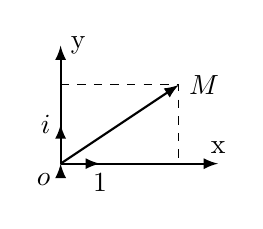
\begin{tikzpicture}[scale=0.5]
	\draw[-latex, thick] (0,0) -- (4,0)node[above]{x};
	\draw[-latex, thick] (0,0) -- (0,3)node[right]{y};
	\draw[-latex, thick] (0,0)node[below left]{$o$};
	
	\draw[-latex, thick] (0,0) -- (0,1)node[left]{$i$};
	\draw[-latex, thick] (0,0) -- (1,0)node[below]{$1$};
	\draw[-latex, thick] (0,0) -- (3,2)node[right]{$M$};
	\draw[dashed] (0,2) -- (3,2) -- (3,0);
\end{tikzpicture}}
\parbox{9cm}{
	Згідно з теорією векторів на площині
	вектори $1=(1,0)$ та $i = (0,1)$ можуть
	слугувати базисом, тоді алгебраїчна форма
	комплексного числа $z$ є саме розкладом $z$
	за цим базисом: $z = x1 + yi$, де $i^2 = -1$.
}

\begin{definition}
	Комплексне число $x - iy$ називається спряженим до комплексного
	числа $z = x + iy$. та позначається символом $\overline{z}$, тобто $\overline{z} = x - iy$.
\end{definition}

Зазначимо, що числу $\overline{z}$ на координатній площині відповідає точка,
симетрична точці $z$ відносно дійсної осі.

\underline{Властивості спряжених чисел}

\begin{enumerate}
	\item $\overline{z_1+z_2} = \overline{z_1} + \overline{z_2}$.
	\item $z + \overline{z} = 2 \text{Re}z$.
	\item $|\overline{z}| = |z|$.
	\item $\overline{z_1z_2} = \overline{z_1}\overline{z_2}$.
	\item $z\overline{z} = |z|^2$.
	\item $z = \overline{z} \Leftrightarrow z \in \mathbb{R}$.
\end{enumerate}

Поділити одне комплексне число $z_1$ на інше комплексне число $z_2$ означає, що
потрібно знайти таке комплексне число $z$, що $z_1 = z_2z$. На практиці ділення 
комплексних чисел виконують за допомогою операції множення: домножують
чисельник і знаменник на число, спряжене знаменнику.

$$\text{Приклад: }\dfrac{1-i}{1+i} = \dfrac{(1-i)^2}{(1-i)(1+i)} = \dfrac{1 - 2i + i^2}{1-i^2} = -\dfrac{2i}{2} = -i.$$

Асоціативний закон множення дозволяє ввести поняття натурального степеня
комплексного числа: $z^n = \underbrace{z \cdot z \cdot ... \cdot z}\limits_n$. За угодою $z^0 = 1$.

Запишемо степені уявної одиниці: $i^0 = 1$, $i^1 = i$, $i^2 = -1$, $i^3 = -i$, $i^4 = 1$.

Останню рівність використовуємо при обчисленні довільних степенів уявної
одиниці.

Приклад: $i^{19} = i^{16 + 3} = i^{16} i^{3} = (i^4)^4i^3 = i^3$.

Множина комплексних чисел позначається $\mathbb{C}$. Очевидно, що множина
дійсних чисел є підмножиною $\mathbb{C}$.

\section{Тригонометрична форма комплексного числа}

Нехай $z \in \mathbb{C}$ і $z \neq 0$.

\begin{definition}
	Озн. Кут $\varphi$ між вектором $z$ і ортом дійсної осі називається аргументом
	комплексного числа $z$ і позначається $\text{Arg}z = \varphi$.
\end{definition}

\parbox{3cm}{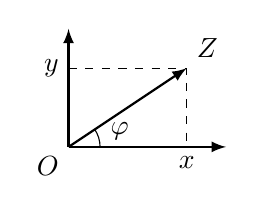
\begin{tikzpicture}[scale=0.5]
	\draw[-latex, thick] (0,0) -- (4,0);
	\draw[-latex, thick] (0,0) -- (0,3);
	\draw (0,0)node[below left]{$O$};
	
	\draw[-latex, thick] (0,0) -- (3,2)node[above right]{$Z$};
	\draw[black] (0.8,0) arc (0:34:0.8);
	\draw (1.3,0.4)node{$\varphi$};	
	\draw[dashed] (0,2)node[left]{$y$} -- (3,2) -- (3,0)node[below]{$x$};
\end{tikzpicture}}
\parbox{9cm}{
Аргумент визначається неоднозначно з точністю до $2\pi$.
Приймаючи до уваги зв'язок між декартовими і
полярними координатами площини $\mathbb{R}^2$, маємо:

$$\begin{array}{l}
	\cos \varphi = \dfrac{x}{\sqrt{x^2 + y^2}} \\
	\sin \varphi = \dfrac{y}{\sqrt{x^2 + y^2}} \\
\end{array}\text{ і }|z| = \sqrt{x^2 + y^2}\text{ або }\begin{array}{l}
	x = |z|\cos\varphi \\
	y = |z|\sin\varphi \\
\end{array}$$
}


Тоді комплексне число $z =x +iy$. можна записати таким чином:
$z = x = |z|(\cos\varphi + i\sin\varphi)$. Ця рівність і називається тригонометричною формою
комплексного числа $z$. 

\begin{problem}
	Записати в тригонометричній формі комплексне число $z = 1 + i$.
\end{problem}
\begin{solution}
	$|z| = \sqrt{1^2 + 1^2} = \sqrt{2}$, $\tg\varphi = \frac{1}{1} = 1$, $\varphi = \frac{\pi}{4}$, оскільки число $z$
	лежить у першій чверті. Отже, $z = 1 + i = \sqrt{2}(\cos\frac{\pi}{4} + i\sin\frac{\pi}{4})$.
\end{solution}

Зауважимо, що дійсні числа теж можна представити як комплексні числа в
тригонометричній формі: $2 = 2(\cos 0 + i\sin 0)$, $-1 = 1(\cos \pi + i\sin \pi)$. 

